\begin{figure}[htbp]
\centering
\begin{subfigure}[b]{0.45\textwidth}
\captionsetup{margin=0cm}  % Remove caption margin for this subfigure
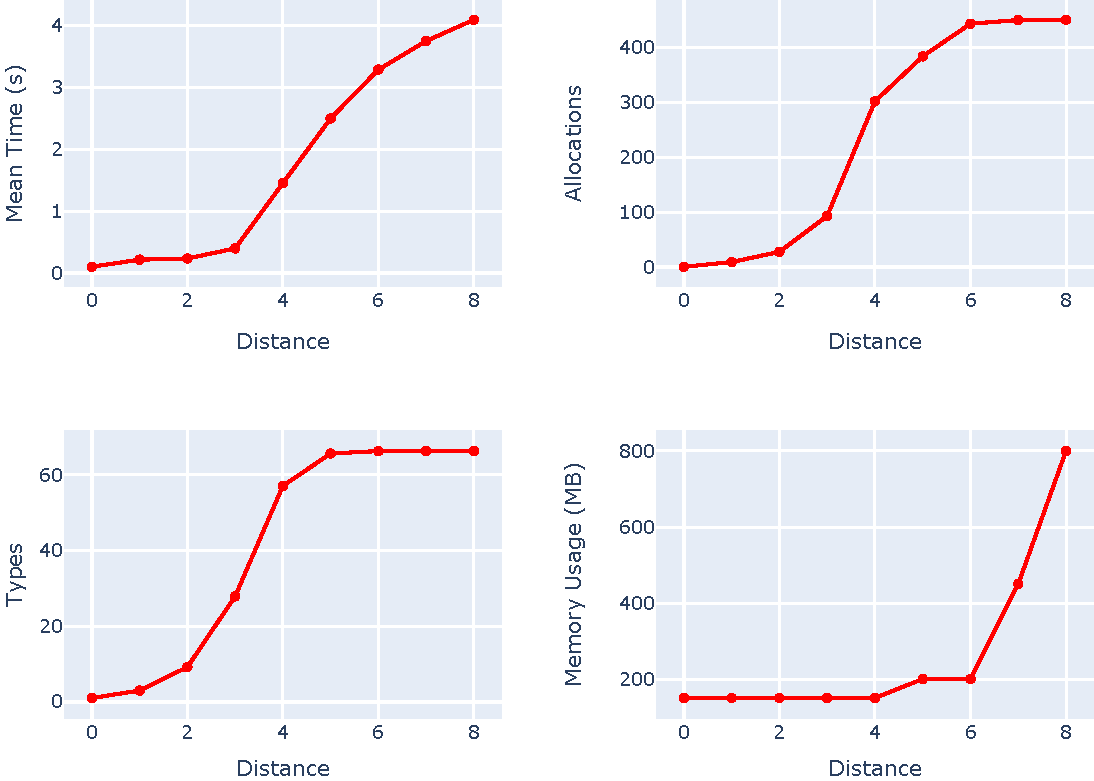
\includegraphics[width=\textwidth]{figures/commons-jxpath_distance_evaluation.pdf}
\caption{commons-jxpath}
\end{subfigure}
\vspace{0.5cm}
\hfill
\begin{subfigure}[b]{0.45\textwidth}
\captionsetup{margin=0cm}  % Remove caption margin for this subfigure
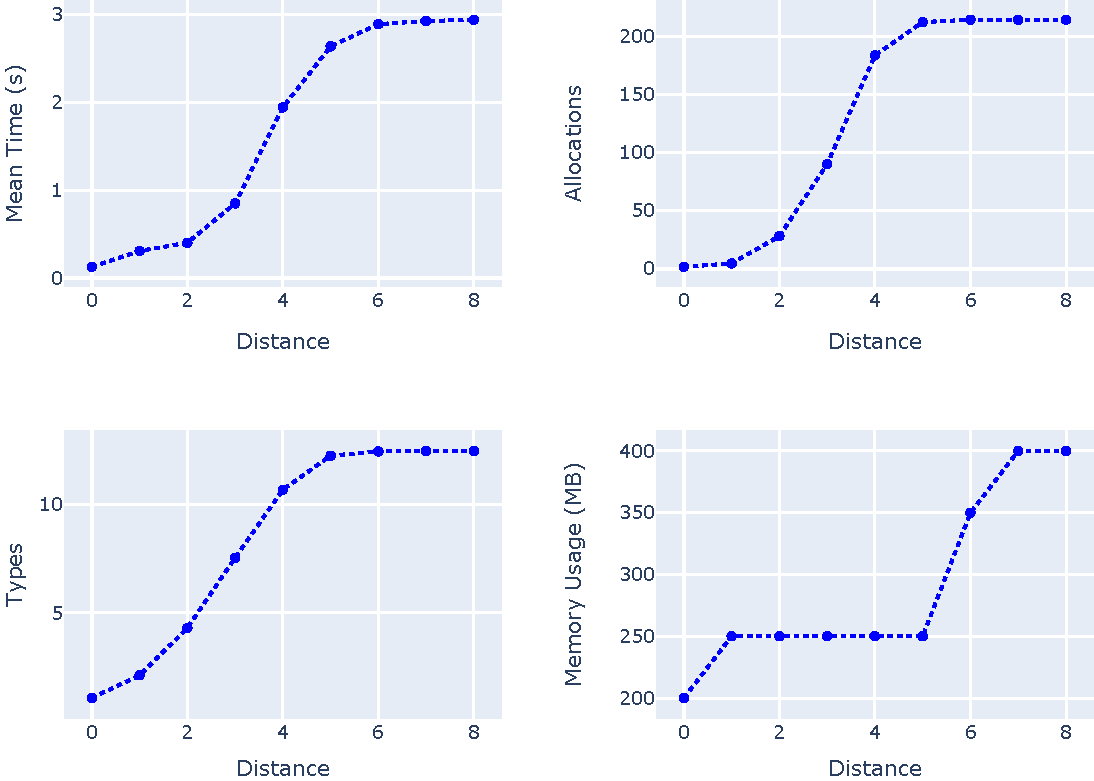
\includegraphics[width=\textwidth]{figures/antlr-2.7.2_distance_evaluation.pdf}
\caption{antlr-2.7.2}
\end{subfigure}
\vspace{0.5cm}
\\
\begin{subfigure}[b]{0.45\textwidth}
\captionsetup{margin=0cm}  % Remove caption margin for this subfigure
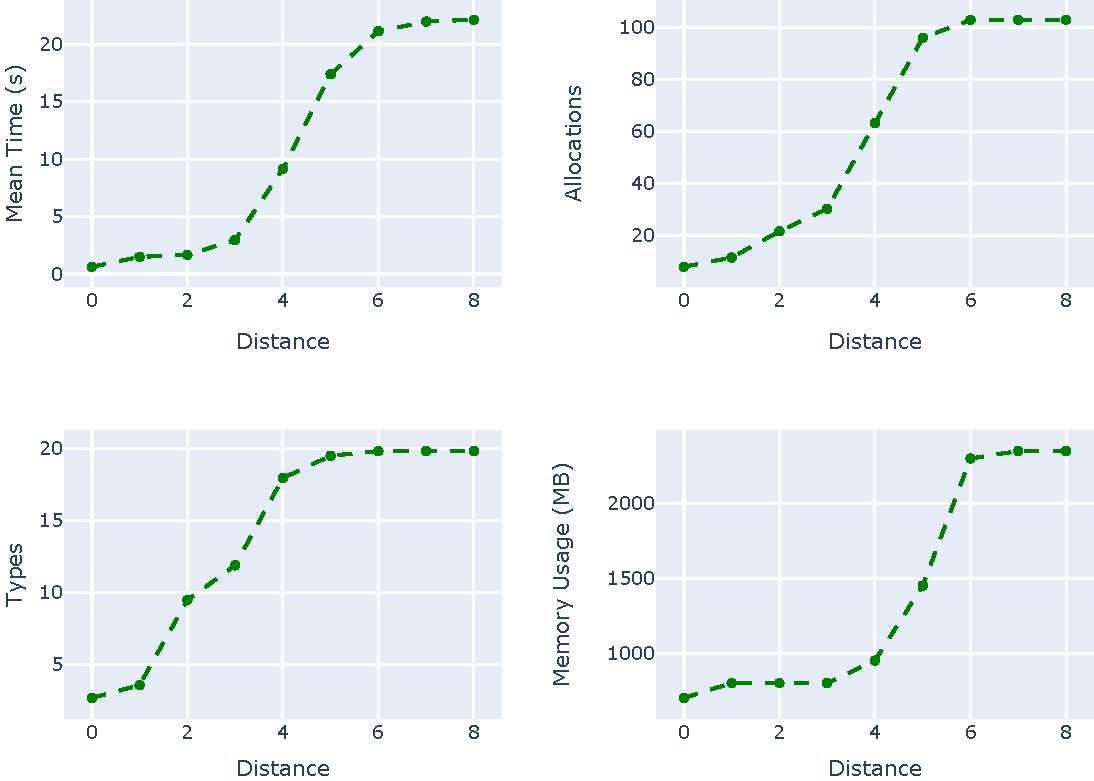
\includegraphics[width=\textwidth]{figures/fop-0.95_distance_evaluation.pdf}
\caption{fop-0.95}
\end{subfigure}
\vspace{0.5cm}
\hfill
\begin{subfigure}[b]{0.45\textwidth}
\captionsetup{margin=0cm}  % Remove caption margin for this subfigure
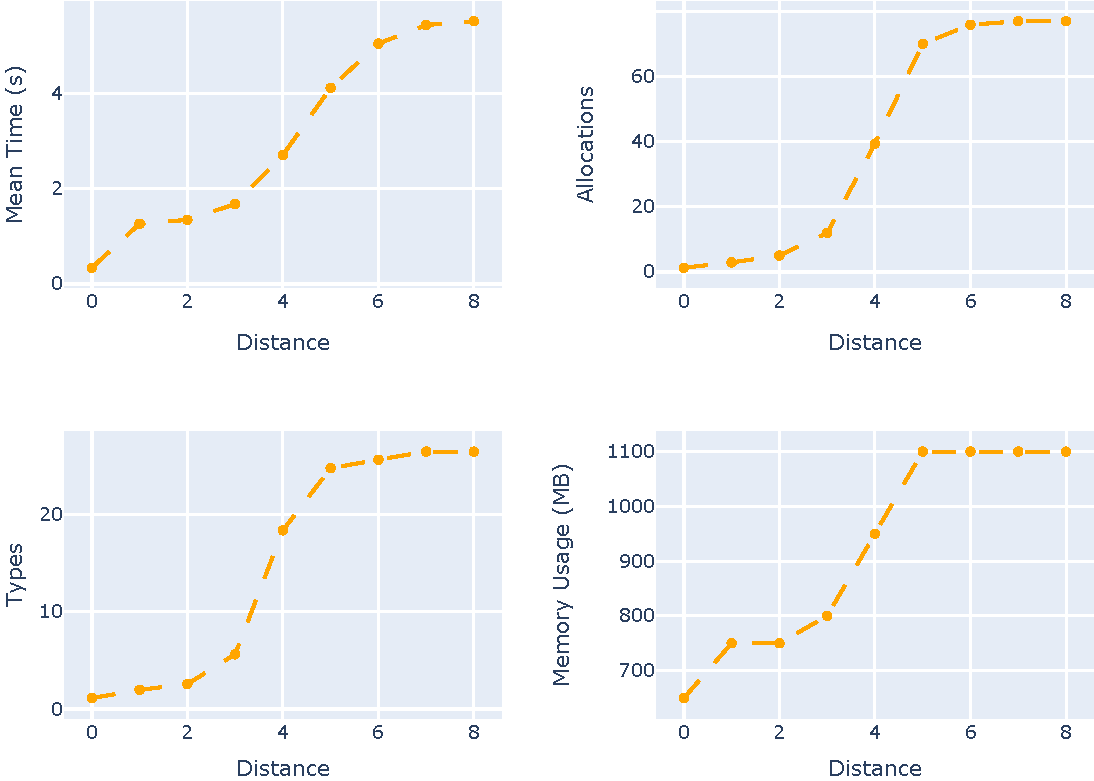
\includegraphics[width=\textwidth]{figures/pmd-4.2.5_distance_evaluation.pdf}
\caption{pmd-4.2.5}
\end{subfigure}
\vspace{0.5cm}
\\
\begin{subfigure}[b]{0.45\textwidth}
\captionsetup{margin=0cm}  % Remove caption margin for this subfigure
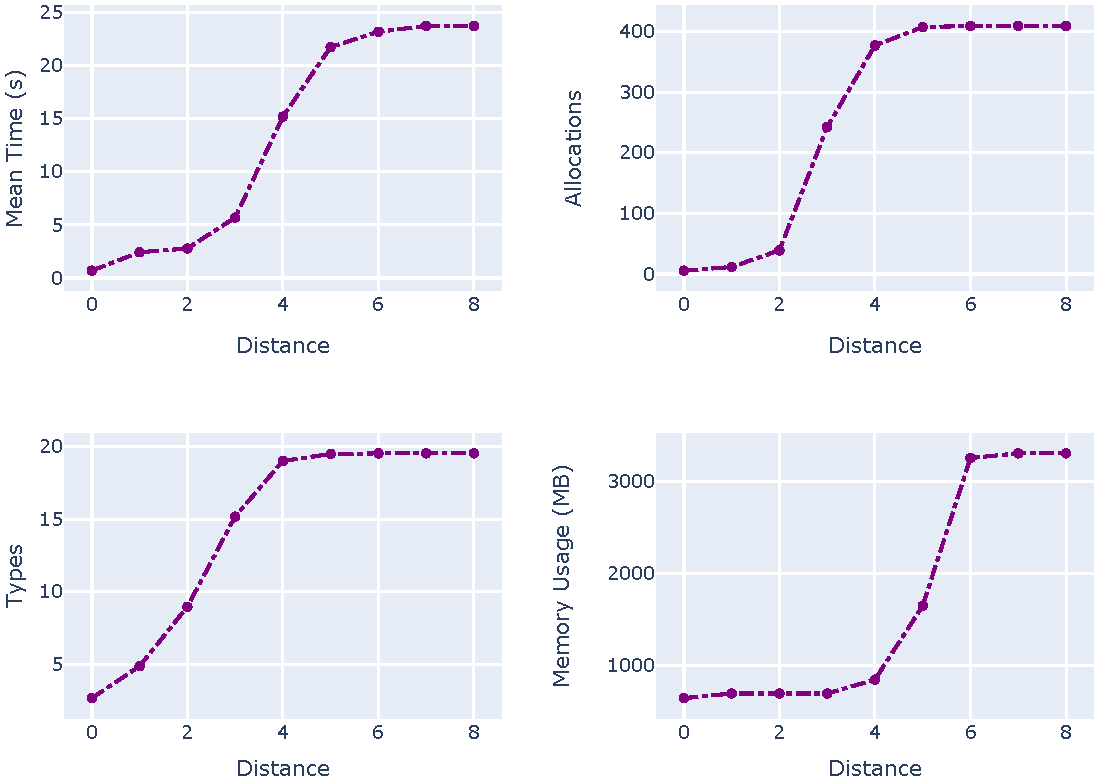
\includegraphics[width=\textwidth]{figures/jfreechart-1.0.0_distance_evaluation.pdf}
\caption{jfreechart-1.0.0}
\end{subfigure}
\vspace{0.5cm}
\hfill
\begin{subfigure}[b]{0.45\textwidth}
\captionsetup{margin=0cm}  % Remove caption margin for this subfigure
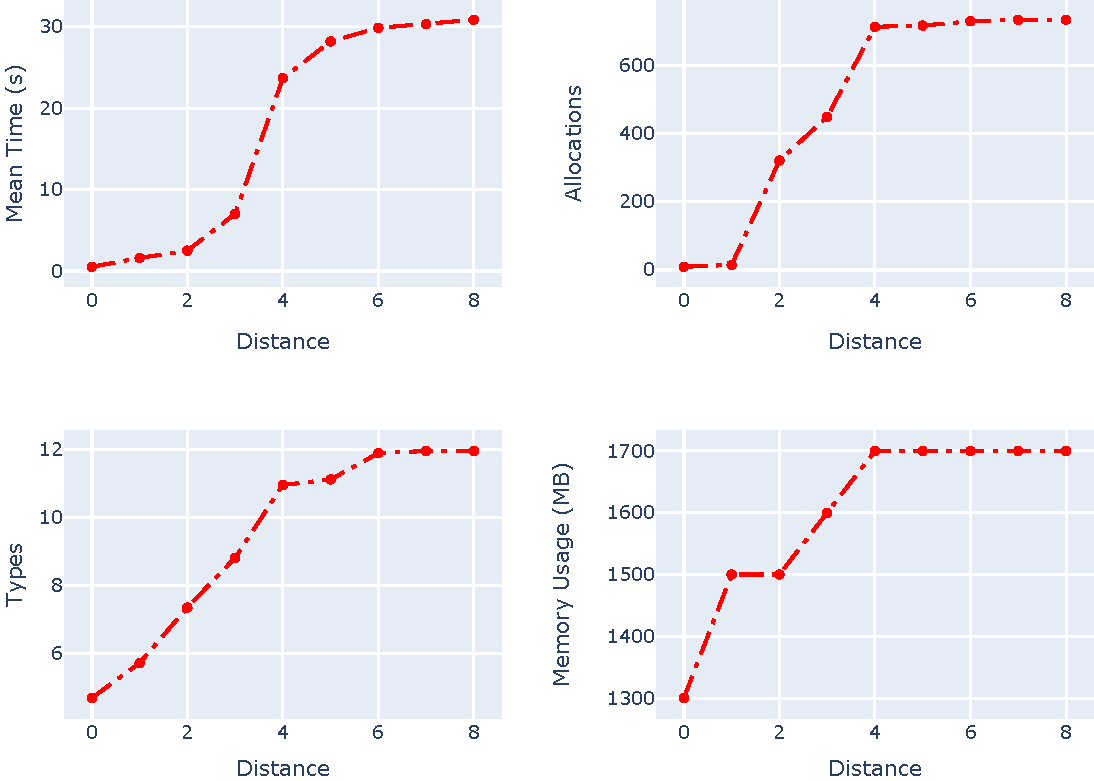
\includegraphics[width=\textwidth]{figures/joda-time_distance_evaluation.pdf}
\caption{joda-time}
\end{subfigure}
\vspace{0.5cm}
\\
\caption{The metrics measured for each dataset. This is the same graphs as shown in Figure~\ref{fig:mean_time}-\ref{fig:memory_usage}, but plotted separately for each benchmark project.}
\label{fig:singles_result}
\end{figure}
